  \begin{section}{Die Konfigurationen}
   Eine Klasse von Graphen ist für den Beweis des Vier-Farben-Satzes wesentlich: Die Konfigurationen. Sie treten vor allem als Untergraphen der normalen Graphen auf. Zuerst wollen wir festhalten, was eine Konfiguration eigentlich ist.
   
   \begin{definitionl}{Konfiguration}{konfig}
    Ein Graph $C$ heißt \textit{Konfiguration}, wenn
    \begin{itemize}
     \item er regulär ist,
     \item die Außenecken einen Ring der Größe größer-gleich 4 bilden,
     \item innere Ecken existieren,
     \item die beschränkten Gebiete von Dreiecken begrenzt werden,
     \item jedes Dreieck Grenze eines Gebiets ist.
    \end{itemize}
   \end{definitionl}
   
   Ein nicht-triviales Beispiel für eine Konfiguration ist der \textit{Birkhoff}-Diamant.
   
    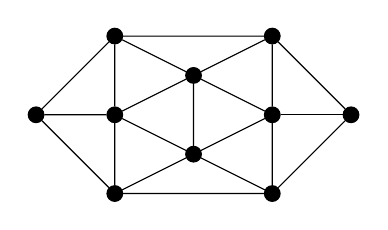
\begin{tikzpicture}[every node/.style={draw,inner sep=2pt,fill=black}]
      \path[shape=circle]
	(0,1) node(a1){} 
	(1,0) node(b1){} (1,1) node(b2){} (1,2) node(b3){}
	(2,0.5) node(c1){} (2,1.5) node(c2){}
	(3,0) node(d1){} (3,1) node(d2){} (3,2) node(d3){}
	(4,1) node(e1){};
	\filldraw (a1) -- (b1) -- (d1) -- (e1) -- (d3) -- (b3) -- (a1) -- (b2);
	\filldraw (b1) -- (b2) -- (b3) -- (c2) -- (d3) -- (d2) -- (d1) -- (c1) -- (b1);
	\filldraw (c1) -- (b2) -- (c2) -- (c1);
	\filldraw (c1) -- (d2) -- (c2);
	\filldraw (d2) -- (e1);
    \end{tikzpicture}
  \end{section}
\newpage